\documentclass[varwidth=\maxdimen]{standalone}

\usepackage{tikz}
\usetikzlibrary{fit}

\tikzset{every label/.style={font=\footnotesize,inner sep=1.5pt}}

\newcommand{\stencilpt}[4][]{\node[circle,draw=blue, label={above:#4},#1] at (#2) (#3) {}}
\newcommand{\stencilptcenter}[4][]{\node[circle,draw=red, label={below:#4},#1] at (#2) (#3) {}}
\begin{document}
	\begin{figure}[h]
		\centering
		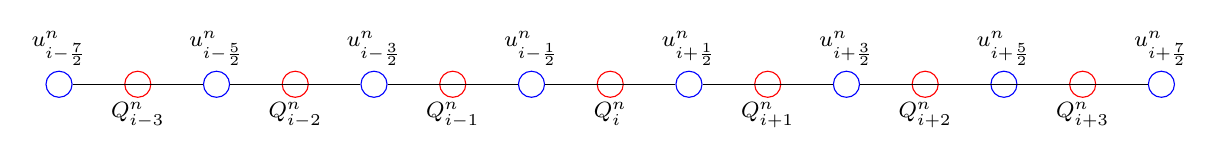
\begin{tikzpicture}
			\stencilpt{-6,0}{i-3}{$u_{i-\frac{7}{2}}^n$};
			\stencilptcenter{-5,0}{k-3}{$Q_{i-3}^n$};
			\stencilpt{-4,0}{i-2}{$u_{i-\frac{5}{2}}^n$};
			\stencilptcenter{-3,0}{k-2}{$Q_{i-2}^n$};
			\stencilpt{-2,0}{i-1}{$u_{i-\frac{3}{2}}^n$};
			\stencilptcenter{-1,0}{k-1}{$Q_{i-1}^n$};
			\stencilpt{ 0,0}{i}  {$u_{i-\frac{1}{2}}^n$};
			\stencilptcenter{ 1,0}{k}{$Q_{i}^n$};
			\stencilpt{ 2,0}{i+1}{$u_{i+\frac{1}{2}}^n$};
			\stencilptcenter{ 3,0}{k+1}{$Q_{i+1}^n$};
			\stencilpt{ 4,0}{i+2}{$u_{i+\frac{3}{2}}^n$};
			\stencilptcenter{ 5,0}{k+2}{$Q_{i+2}^n$};
			\stencilpt{ 6,0}{i+3}{$u_{i+\frac{5}{2}}^n$};
			\stencilptcenter{ 7,0}{k+3}{$Q_{i+3}^n$};
			\stencilpt{ 8,0}{i+4}{$u_{i+\frac{7}{2}}^n$};
			%           \stencilpt{0,-2}{j-2}{$-1/12$};
			%           \stencilpt{0,-1}{j-1}{$4/3$};
			%           \stencilpt[blue]{0, 1}{j+1}{$4/3$};
			%           \stencilpt{0, 2}{j+2}{$-1/12$};
			\draw
			(i-3) -- (i-2)
			(i-2) -- (i-1)
			(i-1) -- (i)
			(i)   -- (i+1)
			(i+1) -- (i+2)
			(i+2) -- (i+3)
			(i+2) -- (i+4);		
	
			%\node[fit=(i-3)(i+4), draw=black, inner sep=10pt] {};
		\end{tikzpicture}
		
		\caption{The five point stencil in 1D.} 
		\label{fig:1}  
	\end{figure}
\end{document}